\section{Layout and Outline}
\label{sec:sl-algorithm}
This section discusses how to produce the SchemaLine visualization such as the one in \autoref{fig:sl-overview}. The layout of schemas is generated before their outlines are computed based on the layout information.

\subsection{SchemaLine Layout}
Based on the technical requirements, the layout should satisfy these conditions: 
\begin{enumerate}
	\item \textbf{Horizontal position}. Along the time axis, events should be located accurately at when they happen, if possible. This is to meet Technical Requirement 1 -- event representation.
	\item \textbf{Relative order}. However, to address scalability, events can be shifted horizontally as long as their relative order is maintained: $x(e_1) < x(e_2)$ if and only if $e_1$ happens before $e_2$, where $x(e)$ is the horizontal position of event $e$.
	\item \textbf{Overlap free}. Events and schemas are not allowed to intersect each other.
\end{enumerate}

To meet these conditions, we design a layout algorithm consisting of the following four steps (\autoref{fig:sl-layout-overview}):
\begin{enumerate} 
	\item Order the schemas vertically based on their number of events.
	\item For each schema, locate its events satisfying the aforementioned requirements.
	\item Compact the schemas following the order computed in the first step.
	\item Locate the remaining events that do not belong to any schemas. 
\end{enumerate}

\begin{figure}[!htb]
\centering
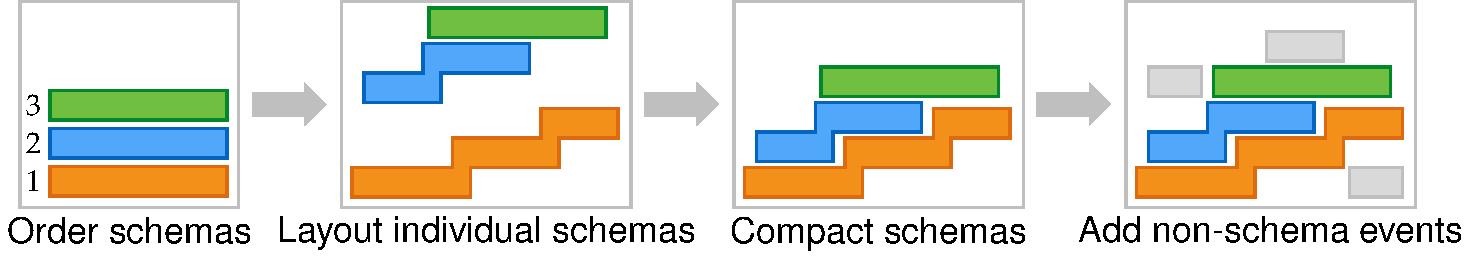
\includegraphics[width=\linewidth]{layout-overview}
\caption{SchemaLine layout algorithm consisting of four steps. First, the vertical order of schemas is computed. Second, the layout of each schema is generated independently. Third, the schemas are compacted based on the computed order. Last, events that do not belong to any schemas are added to the visualization.}
\label{fig:sl-layout-overview}
\end{figure}

\subsubsection{Order Schemas}
As explained in \autoref{sub:schema}, schemas are vertically stacked to apply the \emph{proximity} principle. This step computes the vertical order of all schemas based on their number of events: the schemas with more events are located under the one with less events. This ordering is based on an assumption that larger schemas (in terms of the number of events) are more relevant than smaller ones, thus are located closer to the time axis. If two schemas consist of the same number of events, the one with longer time range is located under.

\subsubsection{Layout Individual Schemas}
\label{sub:layout-schema}
The second step is to produce the layout for each schema. Events that are members of multiple schemas are replicated, allowing the layout of each schema to be generated independently. Events within a schema are sorted chronologically and added to the timeline in that order. Because all events have the same height, only the row level and horizontal position of each event are needed to computed as follows. 

Initially, an event $e_i$ is located on the same row as the previous one $e_{i-1}$ and at the position proportional to its temporal value (Condition 1 -- horizontal position). If these two events are separate, $e_i$ stays at where it is. Otherwise, two cases will be considered. First, if $e_i$ happens at the same time as $e_{i-1}$, it will be located on the upper row and at the same horizontal coordinate as $e_{i-1}$. Second, $e_{i-1}$ is tentatively shifted to the left to make space for $e_i$, as discussed next. If the shift is unsuccessful, $e_i$ will be located in the upper row as in the first case.

\paragraph*{Shifting Events}
To accommodate more events, the accuracy of the horizontal positions of events can be sacrificed. An event can be shifted horizontally to the left to make space for other events. However, an event should not be shifted too far from its accurate position to avoid misinterpretation from analysts. We set that shifting limit to the width of the event so that the event rectangle still covers its time point on the time axis and provides a reasonable indication of its accurate position. 

During shifting, it is essential to make sure that events do not overlap each other (Condition 3 -- overlap free). Considering an event $e_{i-1}$ is shifted to make space for $e_i$, if it overlaps with another event $e_{i-2}$, then $e_{i-2}$ should be shifted as well. Eventually, all events located on the way of the movement should also be shifted. It is also essential to make sure that the relative order between events is still correct after shifting (Condition 2 -- relative order). Otherwise, events with wrong order need to be shifted as well to reestablish the correct order. Note that if two events happen at the same time, they must be located at the same horizontal position. 

\autoref{fig:layout-schema-example} illustrates the layout algorithm for one simple schema.

\begin{figure}[!htb]
	\centering
	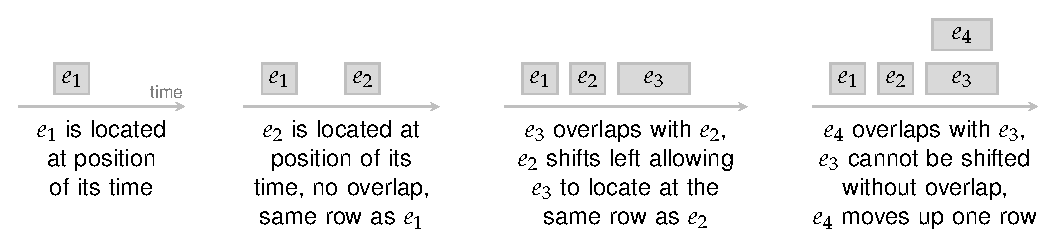
\includegraphics[width=\linewidth]{layout-example}
	\caption{Schema layout algorithm. Four events $e_1$, $e_2$, $e_3$ and $e_4$ are added chronologically.}
	\label{fig:layout-schema-example}
\end{figure}

\subsubsection{Compact Schemas}
This third step stacks schemas in the order computed in the first step to produce an overlap-free visualization. However, to make the layout more vertically compact, it is unnecessary to strictly located schemas in that order. Schemas are processed based on the computed order, starting at the bottom row and moving upward. A schema stops when it does not overlap with previously located schemas. In the worst case, it will be located above all other schemas.

\subsubsection{Add Remaining Events}
This last step allocates events that do not belong to any schemas. Events are sorted chronologically and processed in that order. The ideal horizontal coordinate of an event is the position proportional to its temporal value; however, it can also be shifted using the \emph{shifting} method described earlier in \autoref{sub:layout-schema}. An event begins at the bottom row and moves upward until it does not overlap with any other schemas or events after possible shifts. 

\subsection{Schema Outline}
In this section, we describe a process to produce a polygonal outline covering all the event rectangles of a schema. Only horizontal and vertical line segments are used to keep the outline simple yet aesthetic as in \autoref{fig:schema}. The \emph{polygonal path} $P_n$ of a schema that contains $n$ event rectangles $R_1, R_2, ..., R_n$, ordered from left to right, is determined as follows:
\[
P_n=
\begin{cases}
R_1, & n=1 \\
P_{n-1} \oplus R_n, & n > 1
\end{cases},
\]
where $\oplus$ is an operator that appends a rectangle to a polygonal path. As described in the layout of individual schema (Section \ref{sub:layout-schema}), when a new event is added to an existing schema, it has the same row as the previous event (\autoref{fig:outline-right}) or one row higher (\autoref{fig:outline-up}). To produce an aesthetically pleasing path, two other special cases are also considered as described in \autoref{fig:outline-up-one} and \autoref{fig:outline-up-two}. Technically, a path is represented by a list of vertices and is updated when new events are added. \autoref{fig:sl-outline} illustrates how these vertices are updated, added or unchanged for all four those cases.

\begin{figure}[!htb]
	\centering
	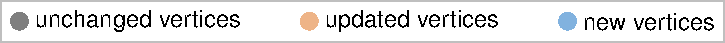
\includegraphics{outline-legend}\bigskip\\
	\subcaptionbox{\label{fig:outline-right}$R_3$ is on the right side of the path.}{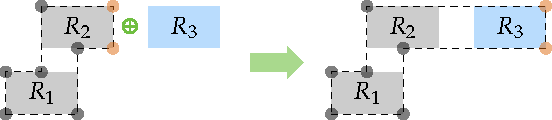
\includegraphics{outline-right}}
	
	\vspace{.5\baselineskip}
	
	\subcaptionbox{\label{fig:outline-up}$R_3$ is on top of the path.}[.43\linewidth]{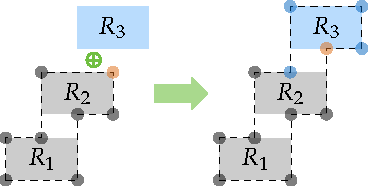
\includegraphics{outline-up}}
	\hfill
	\subcaptionbox{\label{fig:outline-up-one}Left of $R_3$ is a bit greater than left of $R_2$.}[.26\linewidth]{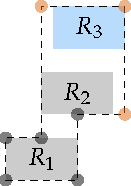
\includegraphics{outline-up-smoothing}}
	\hfill
	\subcaptionbox{\label{fig:outline-up-two}Right of $R_3$ is shorter than right of $R_2$.}[.26\linewidth]{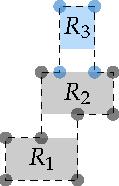
\includegraphics{outline-up-shorter}}
	\caption{Four cases when a new rectangle \colorbox{f2!40}{$R_3$} is appended \textcolor{ForestGreen}{$\pmb{\oplus}$} to a polygonal path -- representing by a dashed polygon. Vertices of the path are colored coded to describe how they are maintained.}
	\label{fig:sl-outline}
\end{figure}

After producing a rectilinear path, all corner bends are made rounded as in \autoref{fig:sl-overview}. The path is filled with the same stroke color but less transparency to make the border stand out with a darker hue. The beginning of the path does not have the border to indicate the flow of events within the path. 